\documentclass[10pt,a4paper]{article}
\usepackage[utf8]{inputenc}
\usepackage[czech]{babel}
\usepackage[T1]{fontenc}
\usepackage{amsmath}
\usepackage{amsfonts}
\usepackage{amssymb}
\usepackage{graphicx}
\usepackage{caption}
\usepackage{subcaption}
\usepackage{placeins}
\usepackage{url}
\usepackage{multirow}
\usepackage[left=2cm,right=2cm,top=3cm,bottom=3cm]{geometry}

\title{Závěrečná zpráva k projektu z Neuronových sítí}
\author{Marie Drábková, Jiří Novotný, Jakub Peschel}


\begin{document}
\maketitle

\section*{Úvod}
Našim cílem je vytvořit neuronovou síť, která rozpoznává, kdo vyhrál v piškvorkách $3\times 3$. Vstupem sítě je finální konfigurace hrací plochy (dále endgame). Výstupem je klasifikace, zda vyhrál  \uv{křížek}, \uv{kolečko} nebo hra skončila remízou. 

Cíl jsme si rozdělili do tří fází. V poslední fázi by síť měla ideálně klasifikovala bitmapový obrázek hrací plochy.


\subsection*{Data}
Téma práce je inspirováno databází UCI Machine Learning \footnote{\url{https://archive.ics.uci.edu/ml/datasets/Tic-Tac-Toe+Endgame}}, ale my jsme se rozhodli klasifikovat i případy výhry \uv{kolečka} a remízy, které databáze nezahrnovala. Proto jsme si vytvořili vlastní generátor endgames v textovém formátu. Dále jsme vytvořili konvertor textových dat do bitmapových obrázků.

Existuje celkem 958 možných endgames. Z nich v 626 případech vyhrál X, v 316 vyhrál O a v 16 hra skončila remízou. Do tréninkových, validačních a testovacích dat jsme data rozdělili v poměru 60:20:20 tak, že v každé množině je stejné procentuální zastoupení vítězství X, O a remíz.

\section*{Implementace}
TODO Jirka: epocha, batchsize, rychlost učení, inicializace vah, chybová funkce, sigmoida, velikost sítě, proč vícevrstvá síť


\section*{Učení}
\subsection*{Textový vstup}
Nejdřív jsme síť naučili na jednoduchém textovém vstupu, který představuje dvourozměrné pole $3\times 3$. Jeho prvky jsou hodnoty z množiny $\{-1,0,1\}$, které reprezentují  postupně \uv{kolečko}, prázdné pole a \uv{křížek}.

Jako první jsme vyzkoušeli velikost sítě (9,9,3), rychlost učení 0,05, 500 epoch. Síť se naučila rozpoznávat hry s přesností 98,4\,\% za cca 60 epoch. Dále byla přesnost stabilní. Ačkoliv cost function nadále klesala, síť se nepřeučovala, viz grafy \ref{fig:1}. Matice zmatenosti \ref{mz1} (R znamená remíza) ukazuje, že se síť dobře rozpoznává vítězství X a O, ale má problém poznat remízu, protože v tréninkových datech se konfigurace znamenající remízu vyskytují příliš málo a síť se je nezvládne naučit. 

\begin{figure}[h!]
\centering
\begin{subfigure}{.5\textwidth}
  \centering
  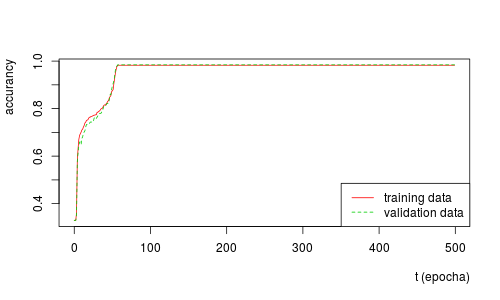
\includegraphics[width=\textwidth]{a1}
  \caption{Accurancy}
  \label{fig:a1}
\end{subfigure}%
\begin{subfigure}{.5\textwidth}
  \centering
  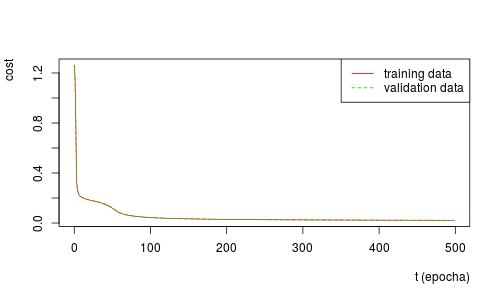
\includegraphics[width=\textwidth]{c1}
  \caption{Cost}
  \label{fig:c1}
\end{subfigure}
\caption{Textový vstup, síť (9,9,3)}
\label{fig:1}
\end{figure}


\shorthandoff{-}
\begin{table}[h!]
\centering
\begin{tabular}{|c|c|c|c|c|}
\hline 
& \multicolumn{4}{c|}{Actual} \\ \cline{2-5}
& & X& O & R\\\hline 
\multirow{3}*{Predicted}& X & 125 & 0 & 3 \\ \cline{2-5}
& O & 0 & 63 & 0 \\ \cline{2-5}
& R &0 & 0 & 0 \\ \hline 
\end{tabular}
\shorthandon{-}
\caption{Matice zmatenosti pro síť (9,9,3) a textový vstup}
\label{mz1}
\end{table}

\FloatBarrier
Poté jsme postupně zkoušeli zmenšovat velikost sítě na (9,3,3) až (9,3). I síť bez vnitřní vrstvy byla schopna dávat stejné výsledky jako výše popsaná síť (9,9,3). Pouze průběh učení byl jiný, viz grafy \ref{fig:2}. Matice zmatenosti vypadá stejně, viz \ref{mz1}. 







\begin{figure}[h!]
\centering
\begin{subfigure}{.5\textwidth}
  \centering
  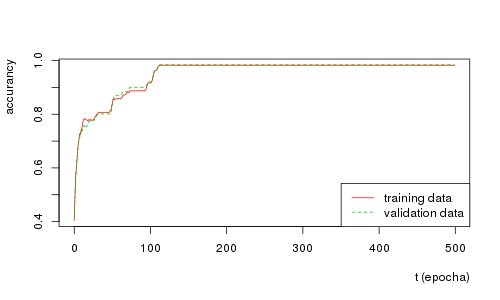
\includegraphics[width=\textwidth]{a2}
  \caption{Accurancy}
  \label{fig:a2}
\end{subfigure}%
\begin{subfigure}{.5\textwidth}
  \centering
  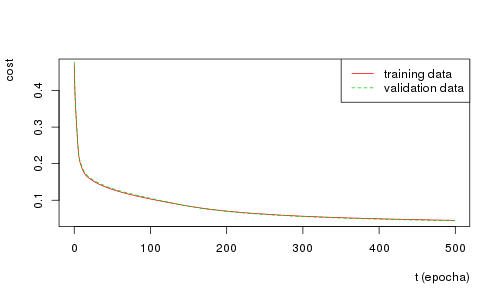
\includegraphics[width=\textwidth]{c2}
  \caption{Cost}
  \label{fig:c2}
\end{subfigure}
\caption{Textový vstup, síť (9,3)}
\label{fig:2}
\end{figure}


Po podrobnějším zkoumání vah jsme dospěli k závěru, že síť považuje za výherce X právě tehdy, když suma na hrací ploše je 1 a pokud je suma 0, považuje za výherce O. Jenomže pokud hrací plocha představuje remízu, suma je taky jedna a síť tuto situaci klasifikuje jako výhru X.

\subsubsection*{Pokus o řešení špatně interpretovaných remíz}
Nejdříve jsme chtěli síti umožnit větší šanci pro naučení remízových stavů, a proto jsme zduplikovali remízové endgames v tréninkové množině. Tato data jsme použili pro trénink sítě velikosti (9,3), ale nic nového se nenaučila. Větší síť (9,9,3) zvýšila svou přesnost na testovací množině z 99,4\,\% na 99,5\,\%. Z matice zmatenosti \ref{mz2} je vidět, že některé případy remízy dokážeme rozpoznat.

\shorthandoff{-}
\begin{table}[h]
\centering
\begin{tabular}{|c|c|c|c|c|}
\hline 
& \multicolumn{4}{c|}{Actual} \\ \cline{2-5}
& & X& O & R\\\hline 
\multirow{3}*{Predicted}& X & 125 & 0 & 1 \\ \cline{2-5}
& O & 0 & 63 & 0 \\ \cline{2-5}
& R &0 & 0 & 2 \\ \hline 
\end{tabular}
\shorthandon{-}
\caption{Matice zmatenosti pro síť (9,9,3) a textový vstup s opakováním na tréninkové množině}
\label{mz2}
\end{table}

\FloatBarrier
\subsection*{Grafický vstup $11\times 11$}
V druhé fázi jsme síti předhodili černobílý bitmapový obrázek o velikosti $11\times 11$ pixelů (viz obrázek \ref{fig:v1}).


\FloatBarrier
\subsection*{Grafický vstup $14\times 14$}
(viz obrázek \ref{vzor14}).

\begin{figure}[h!]
\centering
\begin{subfigure}{.5\textwidth}
  \centering
  %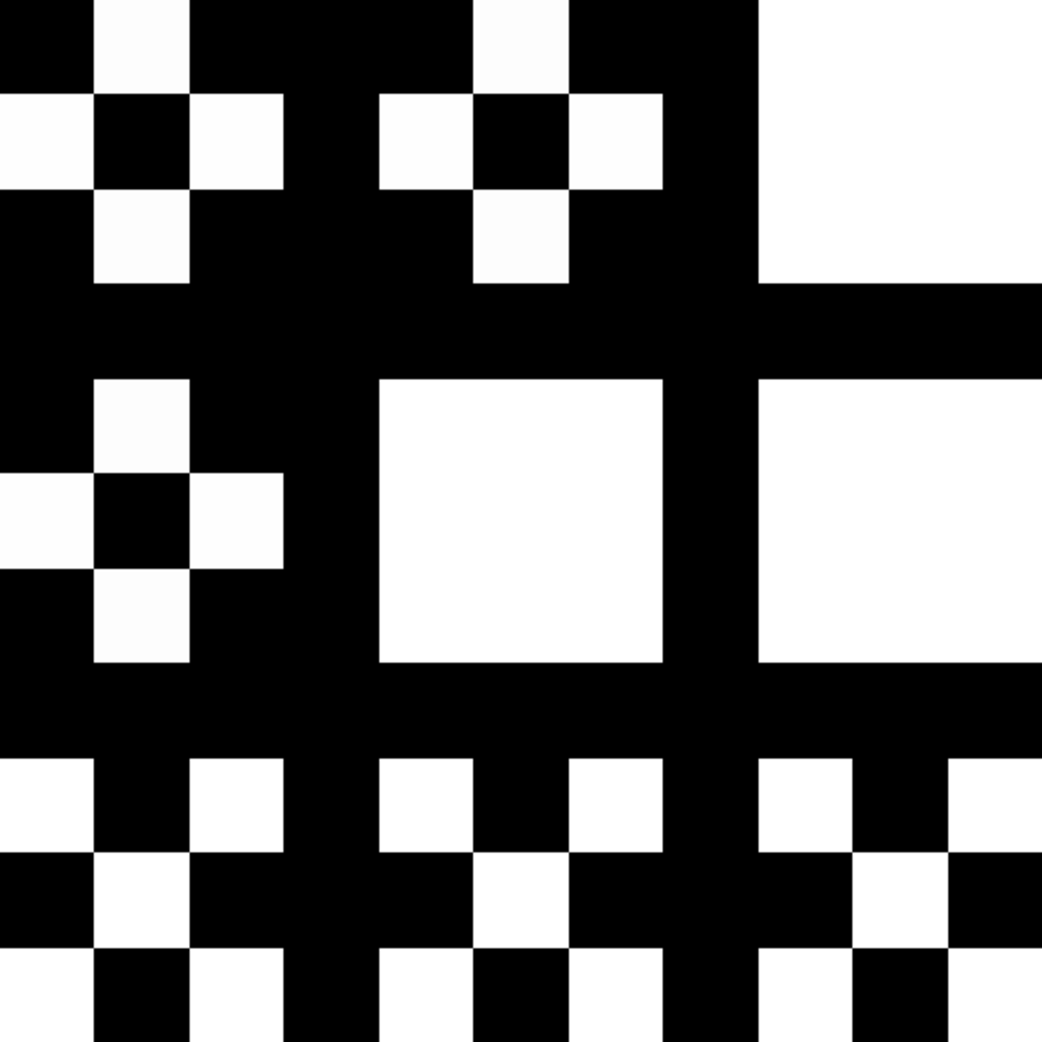
\includegraphics[scale=0.2]{vzor11}
  \caption{$11\times 11$}
  \label{fig:v1}
\end{subfigure}%
\begin{subfigure}{.5\textwidth}
  \centering
  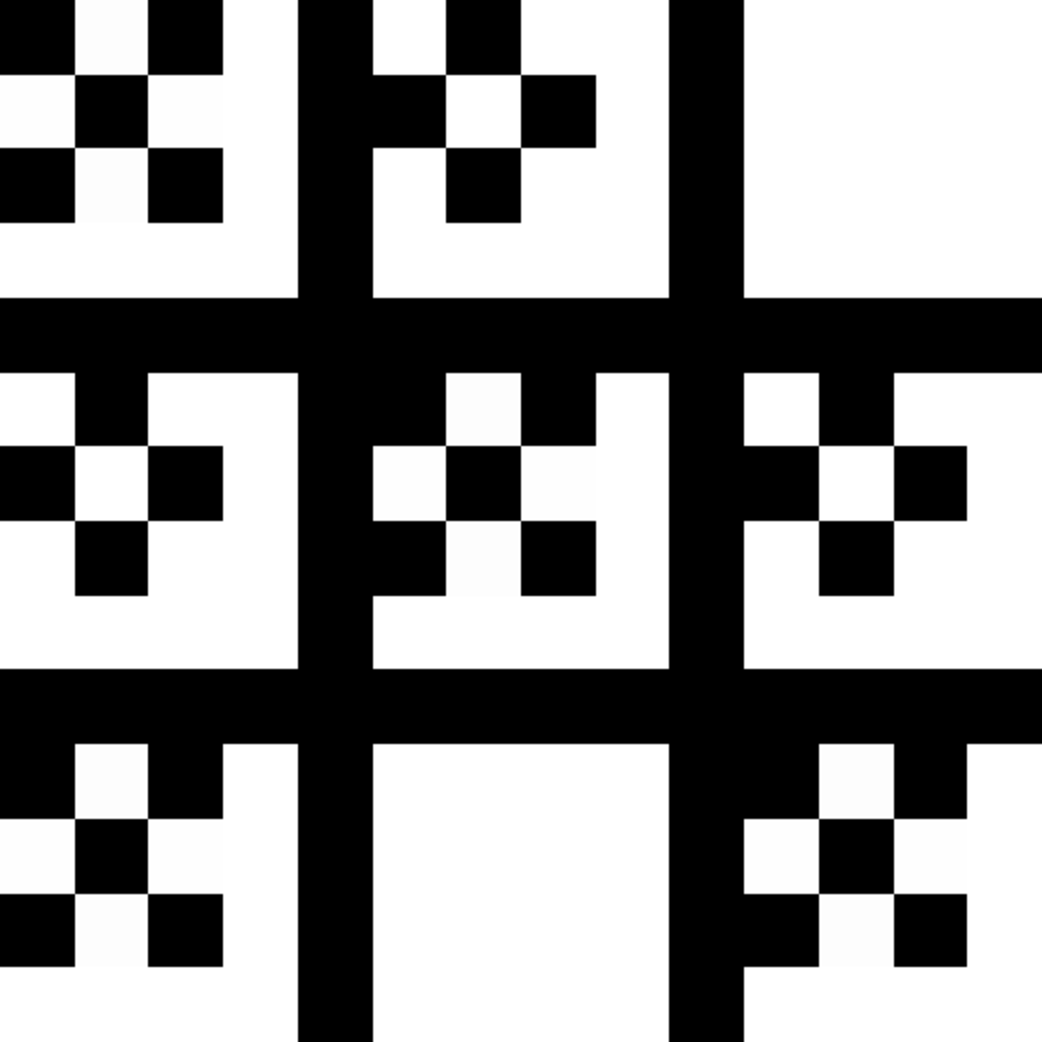
\includegraphics[scale=0.2]{vzor14}
  \caption{$14\times 14$}
  \label{fig:v2}
\end{subfigure}
\caption{Vzorový grafický vstup}
\label{fig:v}
\end{figure}

\FloatBarrier
\section*{Přínosy členů týmu}
Marie Drábková vytvořila generátor endgames a zabývala se rozdělením dat do tréninkových, validačních a testovacích množin. 
Jiří Novotný se postaral o vlastní implementaci sítě.
Jakub Peschel vytvořil konvertor textových dat do bitmapových obrázků.
Učení sítě jsme prováděli společně ve skupině.
Závěrečnou zprávu napsali Jiří Novotný a Marie Drábková.

\section*{Závěr}
TODO

Síť jsme naučili piškvorky pro textový a jednoduchý grafický vstup. Pro složitější vstup je to problematické a možná by se hodila jiná síť.

\end{document}